%\pagenumbering{arabic}

\section{Memory Management}
\subsection{Physical Page Management}
\subsubsection{Homework \Rmnum{3}}
\begin{flushleft}
{\Large Question}
\end{flushleft}

In the file kern/pmap.c, you need to implement the code for the following function (see below, given in order):

Boot\_alloc()

Mem\_init() (before calling check\_page\_free\_list(1))

Page\_init()

Page\_alloc()

Page\_free()

Check\_page\_free\_list() and check\_page\_alloc() will test your physical page allocator. You need to guide JOS

Then check the success report for check\_page\_alloc(). It would be helpful to add your own assert() to verify that your assumptions are correct.
\begin{flushleft}
{\Large Theoretical preparation}
\end{flushleft}


The operating system must keep track of which memory regions are free and which are occupied. The JOS kernel manages memory with the minimum granularity of pages (pages), which uses the MMU to map and protect the memory allocated for each block.

Here we have to write the allocation subfunction of the physical memory page. It uses a linked list of structure PageInfo to record which pages are free, and each node in the linked list corresponds to a physical page.

\begin{flushleft}
{\Large Analysis \& Answer}
\end{flushleft}

First, let's look at the structure of PageInfo. From the comments we can see that pp\_link points to Next page on the free list.pp\_ref is the count of pointers (usually in page table entries) to this page, for pages allocated using page\_alloc. Pages allocated at boot time using pmap.c's
Boot\_alloc do not have valid reference count fields.
\begin{figure}[H]
\centering
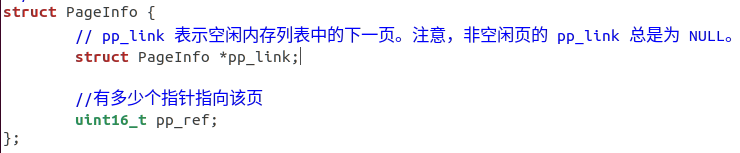
\includegraphics[width=0.8\linewidth]{figure/PageInfo}
\caption{PageInfo}
\end{figure}

We enter the pmap.c file, we can find the mem\_init function, this sub-function will be called when the kernel starts running, and some initialization settings are set for the memory management system of the whole operating system, such as setting the page table and so on. In this function, we can see that the first step is to execute the i386\_detect\_memory function. According to the comment, we can know that it is used to detect how much memory space is available in the system.
\begin{figure}[H]
\centering
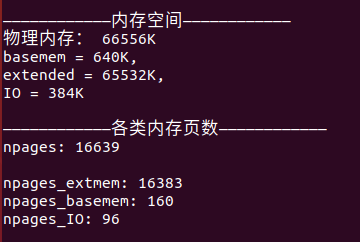
\includegraphics[width=0.8\linewidth]{figure/i386_detect_memory}
\caption{i386\_detect\_memory}
\end{figure}

Jos divides the entire physical memory space into three parts:

One is from 0x00000~0xA0000, this part is also called basemem, which is available.

This is followed by 0xA0000~0x100000. This part is called IO hole and is not available. It is mainly used to allocate to external devices.

This is followed by 0x100000~0x. This part is called extmem and is available. This is the most important memory area.

This sub-function includes three variables, where npages records the total number of pages in memory, npages\_basemem records the number of pages in basemem, and npages\_extmem records the number of pages in extmem.

After executing this function, the next instruction is:

Kern\_pgdir = (pde\_t *) boot\_alloc(PGSIZE);

Memset(kern\_pgdir, 0, PGSIZE);

Where kern\_pgdir is a pointer, pde\_t *kern\_pgdir, which is a pointer to the operating system's page directory table. When the operating system is working in virtual memory mode, the page directory table is required for address translation. The memory size space we allocate for this page directory table is PGSIZE, which is the size of one page. And first clear this part of the memory.
\begin{figure}[H]
\centering
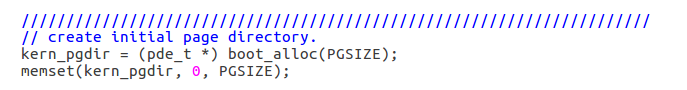
\includegraphics[width=0.8\linewidth]{figure/kern_pgdir}
\caption{kern\_pgdir\&memset}
\end{figure}


As the comment says, this function works as Allocate a chunk large enough to hold 'n' bytes, then update nextfree. Make sure nextfree is kept aligned to a multiple of PGSIZE. it is only used temporarily as a page allocator, then the real page allocator we use is the page\_alloc() function. The core idea of ​​this function is to maintain a static variable nextfree, which stores the virtual address of the next free memory space that can be used, so every time we want to allocate n bytes of memory, we need to modify this variable. Value.


In boot\_alloc, nextfree is the virtual memory address of the next free memory, which is initialized when nextfree is empty.npages is the number of pages. The available memory size is npages × PGSIZE. According to lab1, KERNBASE is the starting address for allocating memory. If nextfree is greater than the value of KERNBASE + npages × PGSIZE, the pointer address overflows.The modified code is as follows

\begin{figure}[H]
\centering
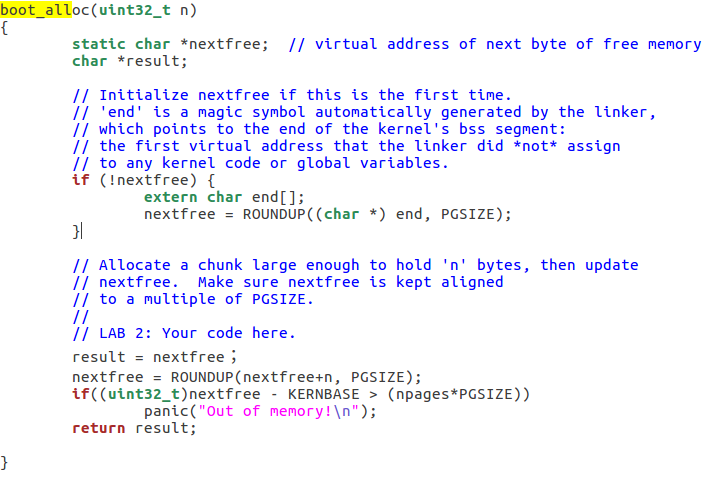
\includegraphics[width=0.8\linewidth]{figure/changed_boot_alloc}
\caption{boot\_alloc}
\end{figure}

Then back to the mem\_init function, we need to add an instruction that asks us to allocate an array of npages 'struct PageInfo's and store it in 'pages'.The kernel uses this array to keep track of physical pages: for each physical page, there is a corresponding struct PageInfo in this array.  'npages' is the number of physical pages in memory.  Use memset to initialize all fields of each struct PageInfo to 0.

We naturally think of the boot\_alloc function that was just completed. By calling it and the memset function, we can complete the required functions. The modified code is as follows:
\begin{figure}[H]
\centering
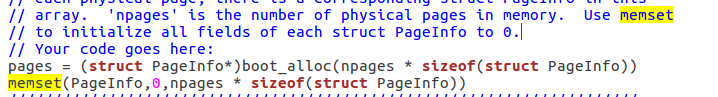
\includegraphics[width=0.8\linewidth]{figure/changed_mem_init}
\caption{mem\_init}
\end{figure}

Referring to the figure below, we can know that the various blocks of memory are as follows:
\begin{flushleft}
I. Physical page 0 is in use for the sake of the fact that we store IDT and
some BIOS structure in it.\\
II. The IO hole (IOPHYSMEM, EXTPHYSMEM) should never be allocated.\\
III. The extended memory, which mainly refer to the memory we allocate to
'pages' and 'kern pgdir' are in use.\\
IV. Then base physical memory are free.\\
\end{flushleft}
\begin{figure}[H]
\centering
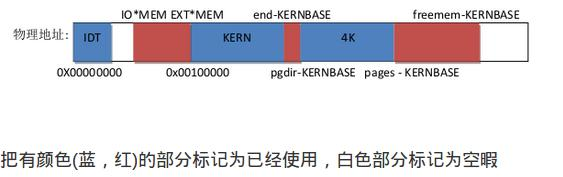
\includegraphics[width=0.8\linewidth]{figure/page_init_pic}
\end{figure}

In the for loop, we determine the state of the current page. If the page is already occupied, set the pp\_ref attribute in the PageInfo structure to one; if it is a free page, then send the page to the pages\_free\_list list, the modified code show as below
\begin{figure}[H]
\centering
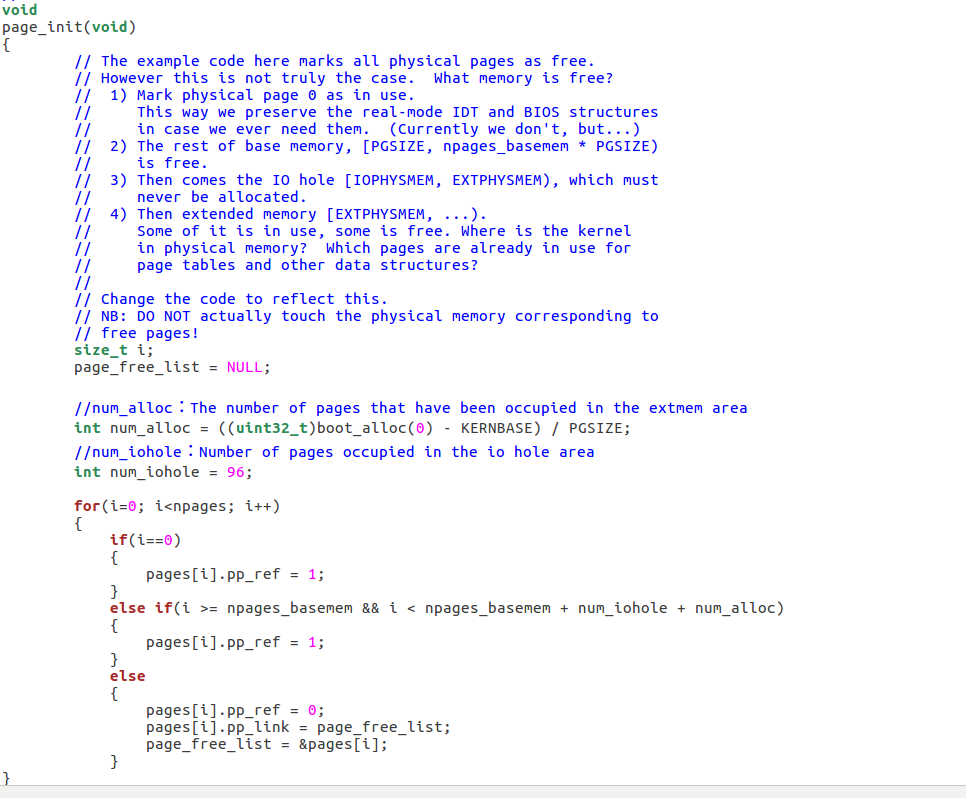
\includegraphics[width=0.8\linewidth]{figure/page_init_changed}
\caption{page\_init}
\end{figure}


Then, we go to implement the page\_alloc function, through the annotation, we know that the function of the function is to allocate a physical page. We can refer to the instructions in the comments to implement it, the implementation code is as follows
\begin{figure}[H]
\centering
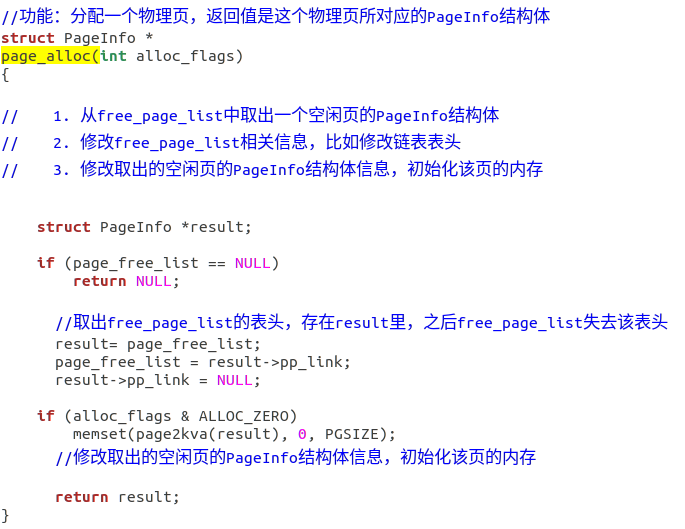
\includegraphics[width=0.8\linewidth]{figure/page_alloc_changed}
\caption{page\_alloc}
\end{figure}

Then, we will complete the page\_free function, we should note that this function should only be called when pp->pp\_ref reach 0. Then, the way we implement it is to add it to the page\_free\_list, the implementation code is as follows
\begin{figure}[H]
\centering
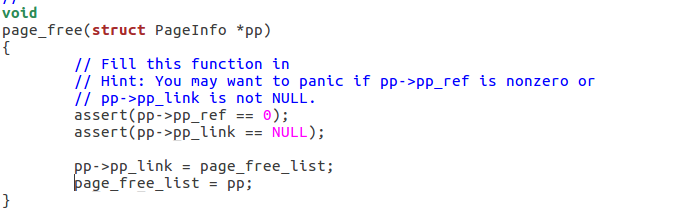
\includegraphics[width=0.8\linewidth]{figure/page_free_changed}
\caption{page\_free}
\end{figure}

\subsection{Virtual Memory}
\subsubsection{Virtual address, linear address and physical address}

In the x86 architecture, a virtual address is composed of two parts, one is a segment selector and the other is a segment offset. A Linear Address refers to an address obtained by converting a virtual address by a segment address translation mechanism. A physical address (Physical Addresses) is the real memory address obtained by the paging address translation mechanism after converting the linear address. This address will eventually be sent to the address bus of your memory chip. The specific relationship of the three addresses is as follows
\begin{figure}[H]
\centering
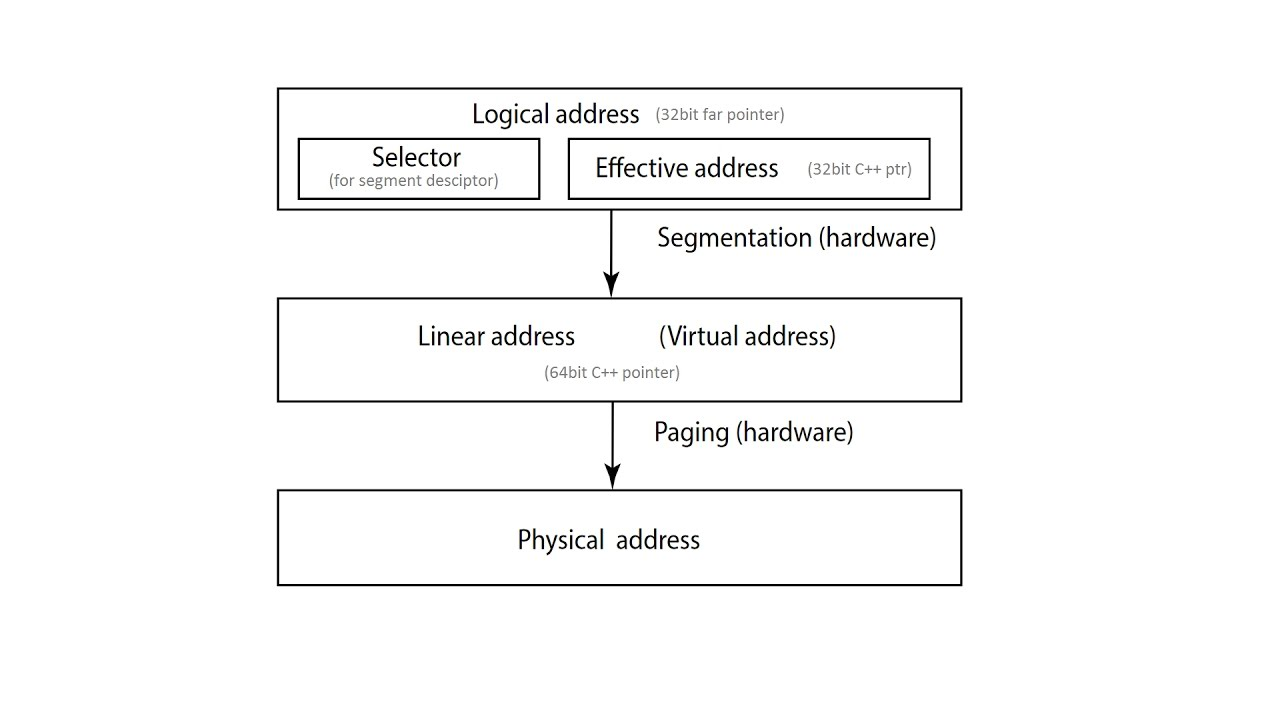
\includegraphics[width=0.8\linewidth]{figure/virtual_linear_physical_address}
\end{figure}

\begin{flushleft}
{\Large Exercise}
\end{flushleft}

GDB can only access QEMU's memory through virtual addresses, but when learning to create virtual addresses, we also need to check the physical address at the same time. Learn QEMU's monitor command, especially the xp command, which allows you to check physical memory.

\begin{flushleft}
{\Large Answer}
\end{flushleft}

Open Terminal, enter qemu-system-i386 -hda obj/kern/kernel.img -monitor stdio -gdb tcp::26000 -D qemu.log , after the correct installation, we can use the monitor command.
\begin{figure}[H]
\centering
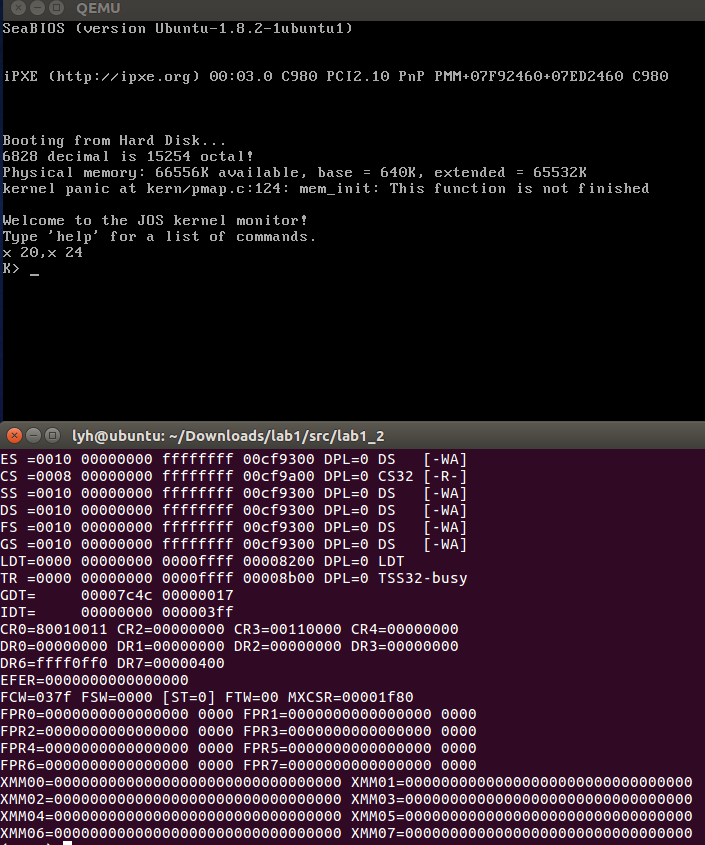
\includegraphics[width=0.8\linewidth]{figure/qemu_commond}
\caption{qemu command}
\end{figure}

\begin{flushleft}
{\Large Exercise}
\end{flushleft}

Assuming the following kernel code is correct, then what type of variable x will be, uintptr\_t or
Physaddr\_t?
\begin{flushleft}
Mystery\_t x;\\
Char* value = return\_a\_pointer();\\
*value = 10; \\
x =(mystery\_t) value;\\
\end{flushleft}
\begin{flushleft}
{\Large Answer}
\end{flushleft}

Since the * operator is used here to resolve the address, the variable x should be of type uintptr\_t.

\subsubsection{Reference counting}
In the previous experiment, we encountered pp\_ref, which records how many different virtual addresses exist on each physical page to reference it. When this value becomes 0, the physical page can be released. In general, the pp\_ref value of any physical page p is equal to the number of times it is mapped by the virtual page under the virtual address UTOP in all page table entries (the address range above UTOP is already mapped at startup) Finished, will not be changed afterwards).

\subsubsection{Page Table Management}
Now we can start writing programs that manage page tables: including inserting and deleting linear address-to-physical address mappings, and creating page tables.

\subsubsection{Homework \Rmnum{4}}
\begin{flushleft}
{\Large Question}\\
In the file kern/pmap.c, you must implement code for the following functions.\\
pgdir\_walk()\\
boot\_map\_region()\\
page\_lookup()\\
page\_remove()\\
page\_insert()\\	
check\_page(), called from mem\_init(), tests your page table management routines. You should make sure it reports success before proceeding.\\
\end{flushleft}
\begin{flushleft}
{\Large Theoretical preparation}
\end{flushleft}

In the previous description, we have a basic understanding of the concept of virtual address, linear address, and physical address.

Physical address: A unit address for memory chip level that corresponds to the address bus to which the processor and CPU are connected.

Logical address: refers to the portion of the offset address associated with the segment generated by the program. For example, in C language pointer programming, you can read the value of the pointer variable itself (\& operation). In fact, this value is the logical address. It is relative to the address of your current process data segment and is not related to the absolute physical address.

Linear address or virtual address:
Similar to the logical address, it is also an unreal address. If the logical address is the corresponding hardware platform segment management pre-conversion address, then the linear address corresponds to the pre-conversion address of the hardware page memory.

We also need to know the knowledge about the page table.

Our physical memory has a total of 4GB, and we assign it to the page, each page is 4KB in size.

The 4GB (2 to the 32th power) linear address space can be divided into 1048576 (2 to the 20th power, that is, 1M, can also be regarded as 1024 * 1024) pages, so you can randomly extract these pages, every 1024 The pages are a group and can be divided into 1024 groups. For each group of 1024 pages of physical addresses, arranged in a certain order can constitute a table (each entry is the physical address of a page), this table is the page table. The size of the page table is 1024*4B=4KB, which is exactly the size of a physical page.

Because it has been divided into 1024 groups, each group has a page table (size 4KB), so these 1024 page tables can be pointed to by a table, this is the page directory. Similar to the page table, the page directory has a total of 1024 entries (called page directory entries), and the content of each page directory entry is the physical address of a page table. The size of the page table is 1024*4B=4KB, which is exactly the size of a physical page.

The conversion of three addresses and the page table mechanism are shown in the figure below.
\begin{figure}[H]
\centering
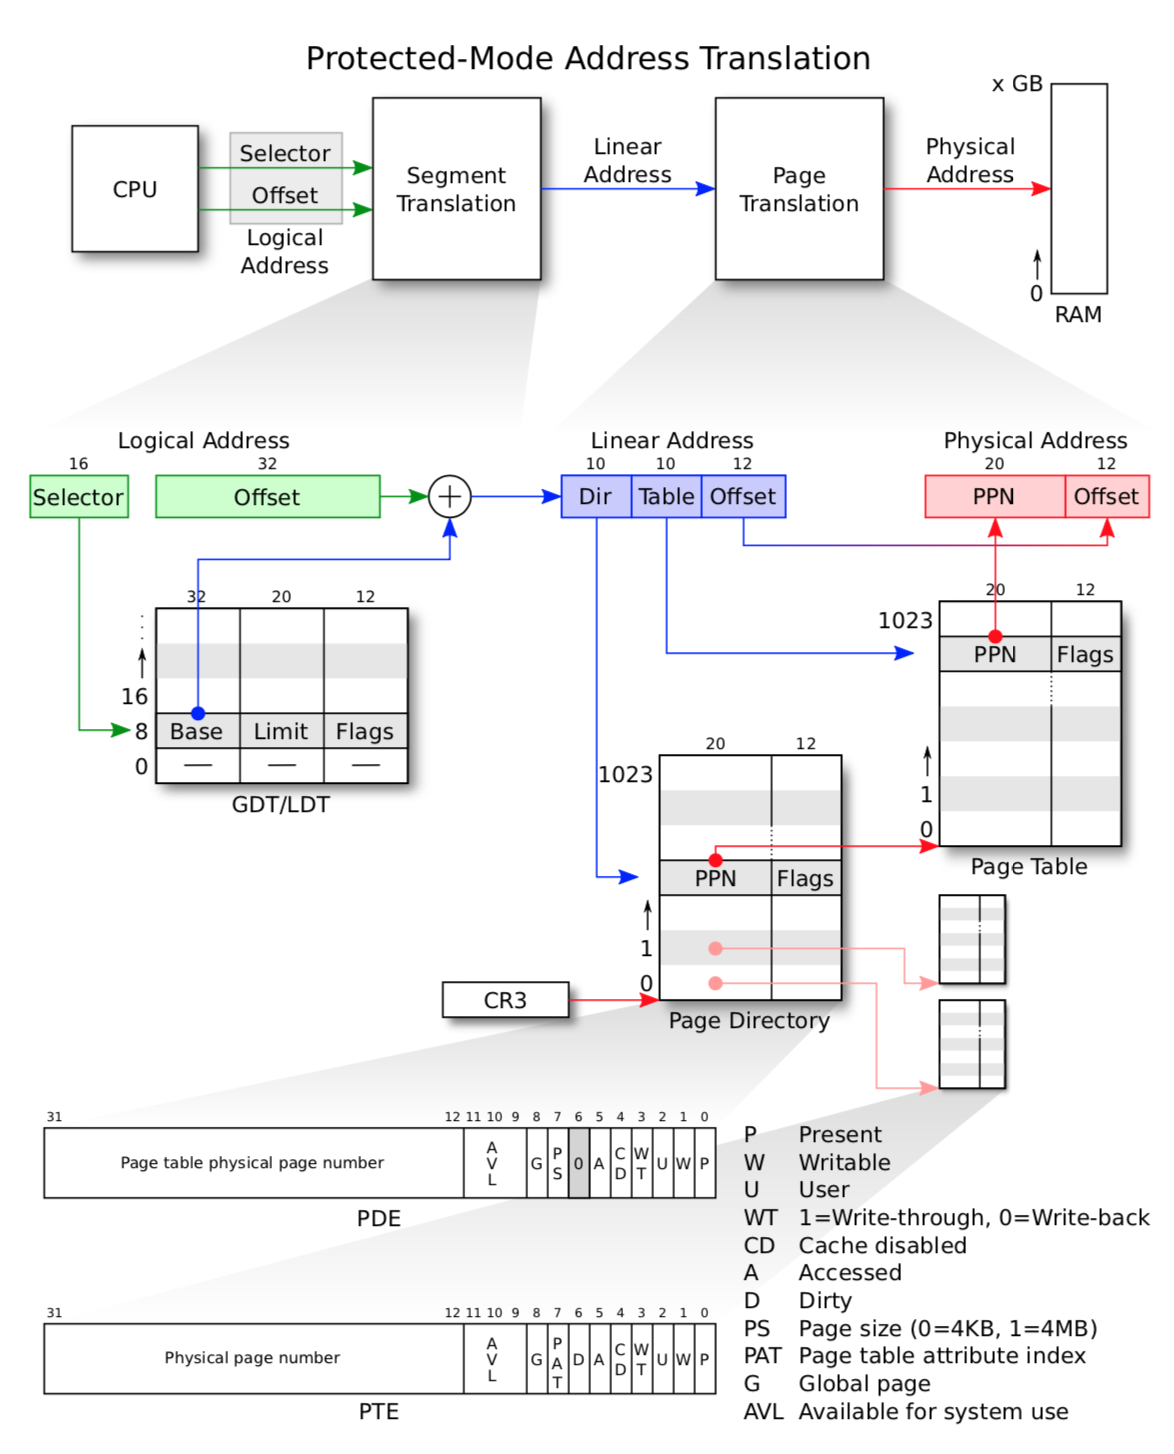
\includegraphics[width=0.8\linewidth]{figure/address_transform}
\end{figure}


\begin{flushleft}
{\Large Analysis \& Answer}
\end{flushleft}

By commenting, we can know that the function of this function is given a page directory table pointer pgdir , which should return the page table entry pointer corresponding to the linear address va.We need to complete the transformation as shown in the figure, return the corresponding page table address, that is, the virtual address of the part circled by the red circle:
\begin{figure}[H]
\centering
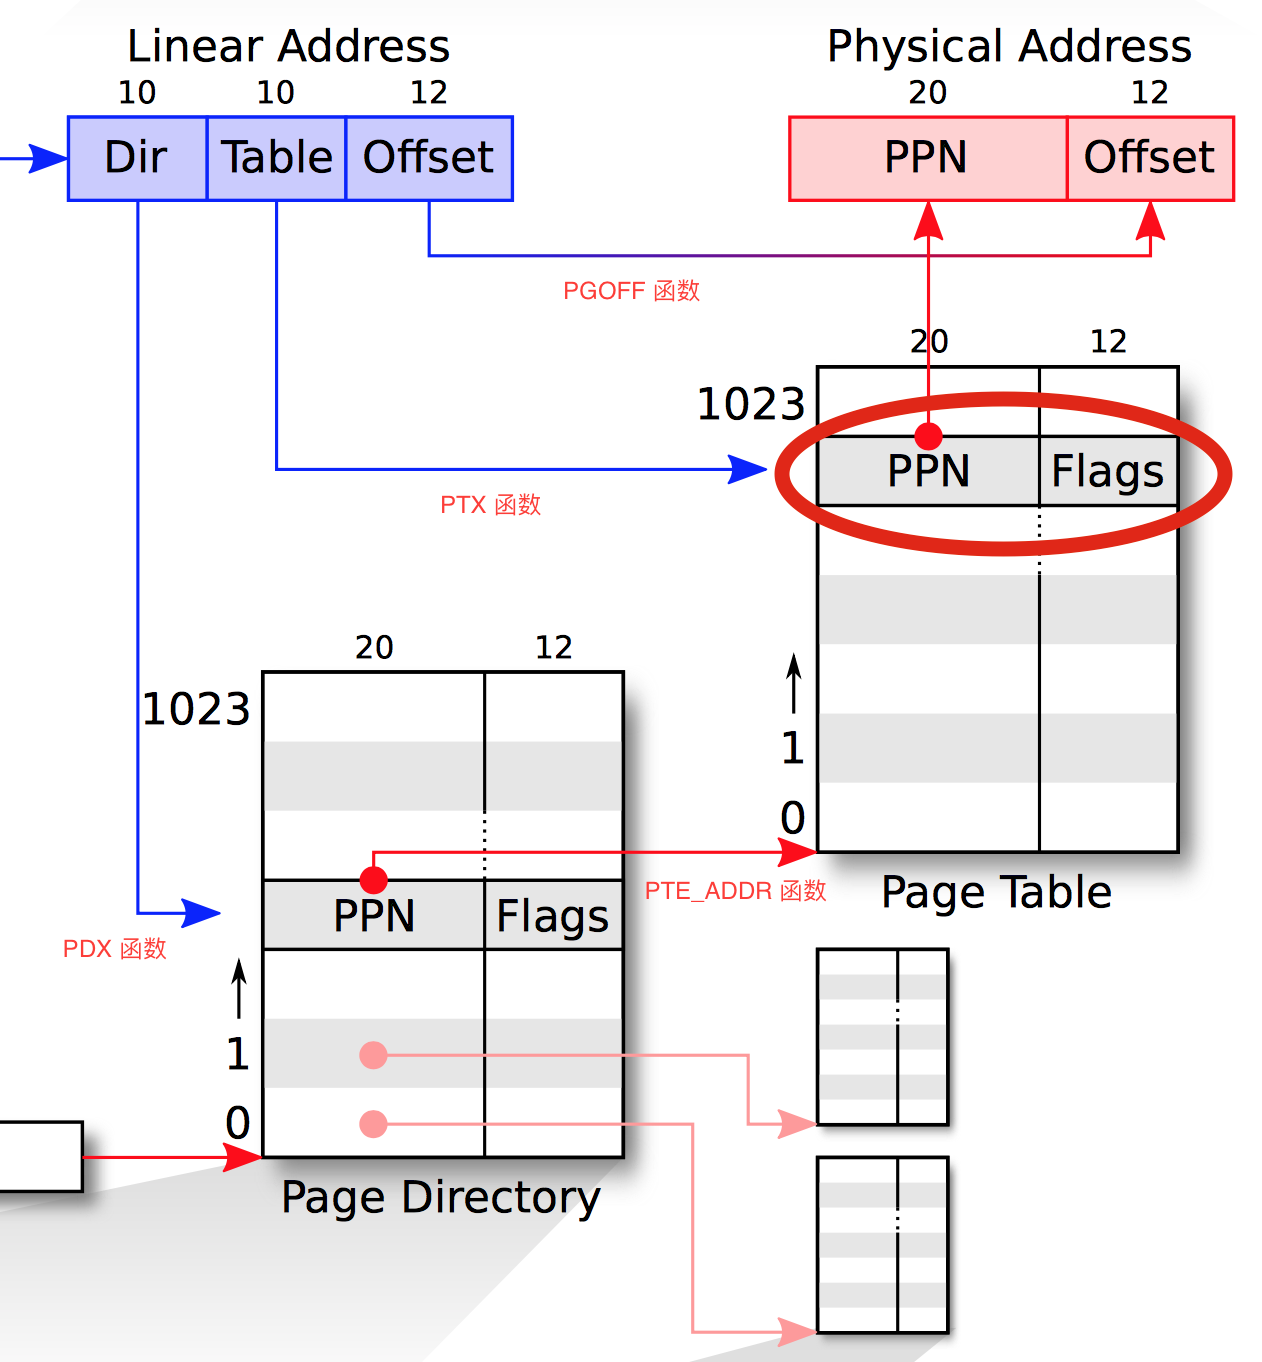
\includegraphics[width=0.8\linewidth]{figure/pgdir_walk_purpose}
\end{figure}

In addition, we need to understand the meaning of the three parameters.In addition, we need to understand the meaning of the three parameters, pgdir means the page directory item pointer, va means linear address, JOS equals virtual address, create means if page directory entry does not exist or not.

Here we should complete the following steps:

1. Find the page table page where the virtual address is located by the page directory table for the page directory entry address dic\_entry\_ptr in the page directory. (7-8)

2. Determine if the page table page corresponding to this page directory entry is already in memory. (10)

3. If yes, calculate the base address page\_base of this page table page, and then return the address of the page entry corresponding to va \&page\_base[page\_off] (23-25)

4. If not, and create is true, a new page is allocated, and the information of this page is added to the page directory entry dic\_entry\_ptr. (11-18)

5. If create is false, it returns NULL. (19-20)

The modified code is shown in the figure
\begin{figure}[H]
\centering
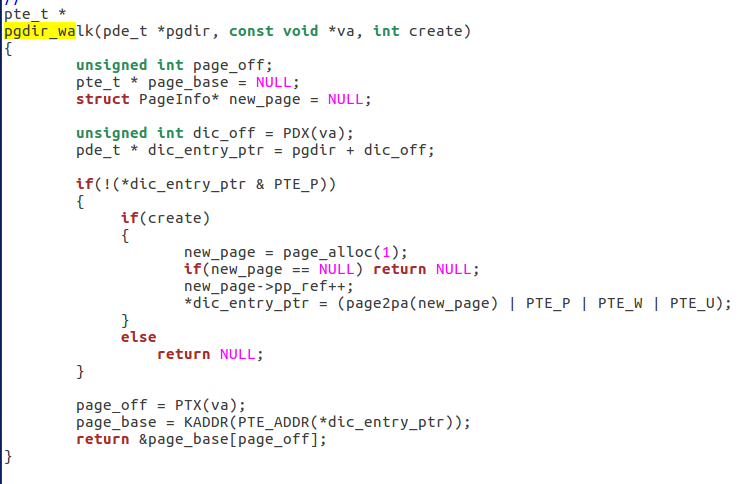
\includegraphics[width=0.8\linewidth]{figure/pgdir_walk_changed}
\caption{pgdir\_walk}
\end{figure}

Next we complete the boot\_map\_region function. By comment, we can see that the function of this function is to map [va, va+size) of virtual address space to physical [pa, pa+size) in the page table rooted at pgdir.  Size is a multiple of PGSIZE,and va and pa are both page-aligned.Use permission bits perm|PTE\_P for the entries.


The mapping of the virtual address space range [va, va+size) to the physical space [pa, pa+size) is added to the page table pgdir. The main purpose of this function is to set the address range above the virtual address UTOP. The address mapping of this part is static and will not change during the operation of the operating system, so the value of the pp\_ref field in the PageInfo structure of this page. No change will happen.

The steps to be completed by this function are as follows:

Need to complete a loop, using the pgdir\_walk function we just completed, we can use a loop to map all the memory in size bytes.The modified code is shown in the figure:
\begin{figure}[H]
\centering
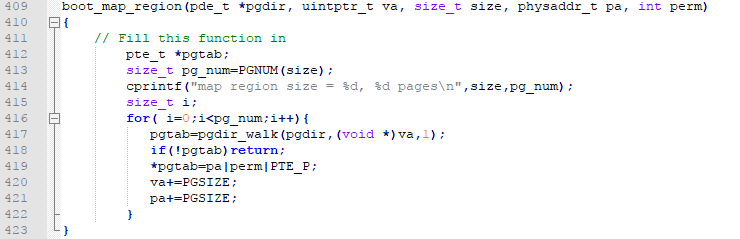
\includegraphics[width=0.8\linewidth]{figure/boot_map_region_changed}
\caption{boot\_map\_region}
\end{figure}

Next, we complete the page\_lookup function, which functions as return the page mapped at virtual address 'va'.If the pte\_store parameter is not 0, the page table entry address of this physical page is stored in pte\_store.

We only need to call the pgdir\_walk function to get the page table entry corresponding to this va, and then determine whether the page is already in memory, and if so, return the PageInfo structure pointer of this page. And store the contents of this page table entry in pte\_store.The modified code is shown in the figure:
\begin{figure}[H]
\centering
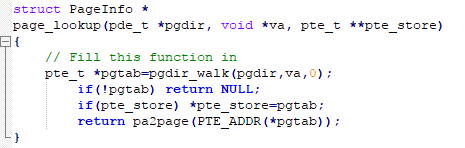
\includegraphics[width=0.8\linewidth]{figure/page_lookup_changed}
\caption{page\_lookup}
\end{figure}

Go ahead and we'll complete the page\_remove function. By commenting, we can know that the function of this function is unmaps the physical page at virtual address 'va'.The modified code is shown in the figure:
\begin{figure}[H]
\centering
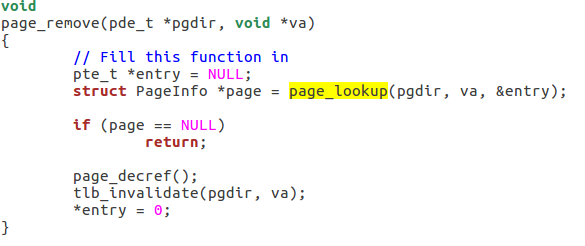
\includegraphics[width=0.8\linewidth]{figure/page_remove_changed}
\caption{page\_remove}
\end{figure}

Go ahead and we'll complete the page\_insert function. By commenting, we can know that the function of the function is map the physical page 'pp' at virtual address 'va'. Combining the previously completed pgdir\_walk function and the page\_remove function, we first find the page table corresponding to the virtual address va through the pgdir\_walk function. Item, modify the value of pp\_ref, check the page table entry, determine whether va has been mapped, if it is mapped, delete the mapping, and add the mapping relationship between va and pp to the page table entry.The modified code is shown in the figure:
\begin{figure}[H]
\centering
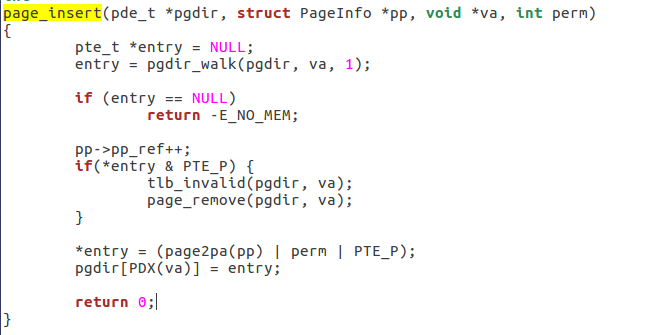
\includegraphics[width=0.8\linewidth]{figure/page_insert_changed}
\caption{page\_insert}
\end{figure}

\subsection{Kernel address space}

JOS divides the 32-bit linear address virtual space into two parts. The user environment (process running environment) usually occupies the part of the low address, called the user address space. The operating system kernel always occupies the part of the high address, called the kernel address space. The dividing line between these two parts is a macro ULIM defined in the memlayout.h file. JOS reserves nearly 256MB of virtual address space for the kernel. This can be understood, why in the experiment 1 to design a high address address space for the operating system. If you don't do this, the address space of the user environment is not enough.

\subsubsection{Homework \Rmnum{5}}
\begin{flushleft}
{\Large Question}
\end{flushleft}
Fill in the missing code in mem\_init() after the call to check\_page().

\begin{flushleft}
{\Large Theoretical preparation}
\end{flushleft}

Since the kernel and user memory are present in the address space of each environment, we need to use the permission bits in the x86 page table to allow the user code to access only the user portion of the address space. Otherwise, bugs in the user code may overwrite the kernel data, causing a crash; or the user code can steal private data from other environments.
The user environment will have no access to any memory above ULIM, and the kernel can read and write this portion of memory. For the address range [UTOP, ULIM), the kernel and the user environment have the same permissions: they can only be read and not written. Under UTOP
The address space is used by the user environment, and the user environment will set permissions to access this part of the memory.
\begin{figure}[H]
\centering
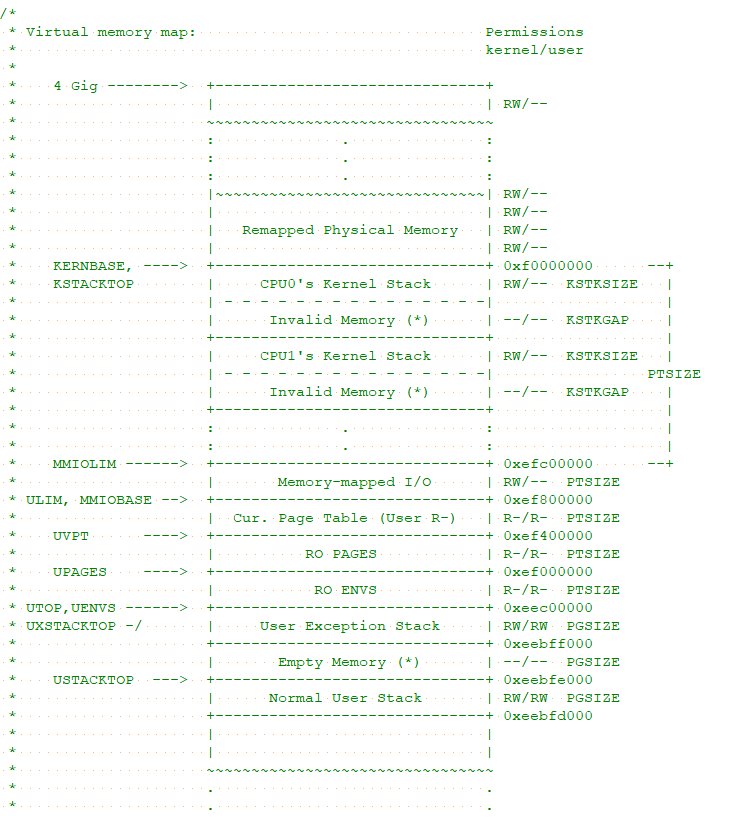
\includegraphics[width=0.8\linewidth]{figure/mem_layout}
\end{figure}

\begin{flushleft}
{\Large Analysis \&Answer}
\end{flushleft}

In this exercise, three virtual addresses are mapped to the physical page.

First, we will complete the UPAGES mapping UPAGES (0xef000000 ~ 0xef400000) up to 4MB, which is the data structure of JOS recording physical page usage.

Currently only one page directory is created, kernel\_pgdir, so the first parameter is obviously kernel\_pgdir. The second parameter is the virtual address, and UPAGES is originally given as a virtual address. The third parameter is the mapped memory block size. The fourth parameter is the physical address mapped to, and the physical address of pages can be taken directly. Permissions PTE\_U indicates that the user has permission to read.Currently only one page directory is created, kernel\_pgdir, so the first parameter is obviously kernel\_pgdir. The second parameter is the virtual address, and UPAGES is originally given as a virtual address. The third parameter is the mapped memory block size. The fourth parameter is the physical address mapped to, and the physical address of pages can be taken directly. Permissions PTE\_U indicates that the user has permission to read.
The modified code is shown in the figure
\begin{figure}[H]
\centering
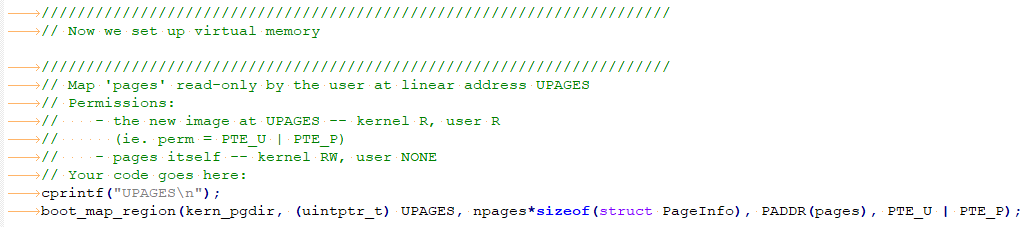
\includegraphics[width=0.8\linewidth]{figure/mem_init_changed1}
\end{figure}


Then there is the memory stack, the kernel stack ( 0xefff8000 ~ 0xf0000000) 32kB
Bootstrap represents the lowest address of the stack. Since the stack grows to the lower address, it is actually the top of the stack. We will map the address space in [KSTACKTOP-KSTKSIZE, KSTACKTOP)
The modified code is shown in the figure
\begin{figure}[H]
\centering
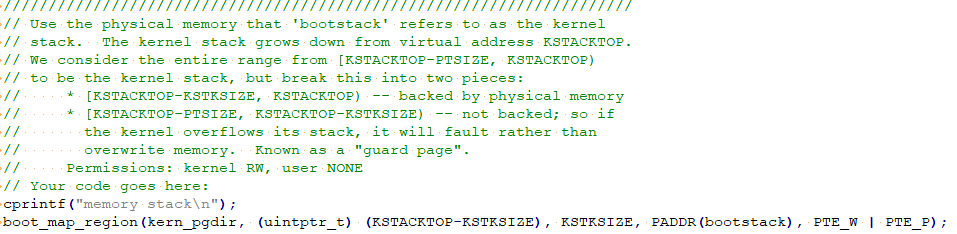
\includegraphics[width=0.8\linewidth]{figure/mem_init_changed2}
\end{figure}


Finally, the kernel part, we will map the kernel ( 0xf0000000 ~ 0xffffffff ) 256MB
The modified code is shown in the figure
\begin{figure}[H]
\centering
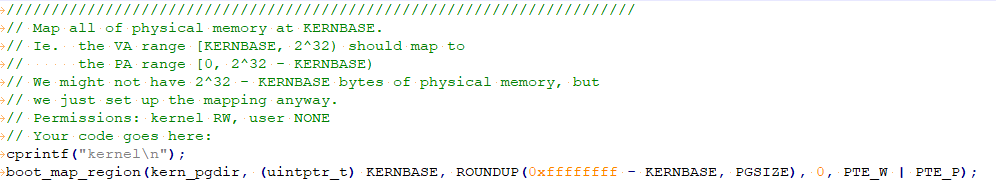
\includegraphics[width=0.8\linewidth]{figure/mem_init_changed3}
\end{figure}

As a result,  the code works successfully.

\begin{figure}[H]
\centering
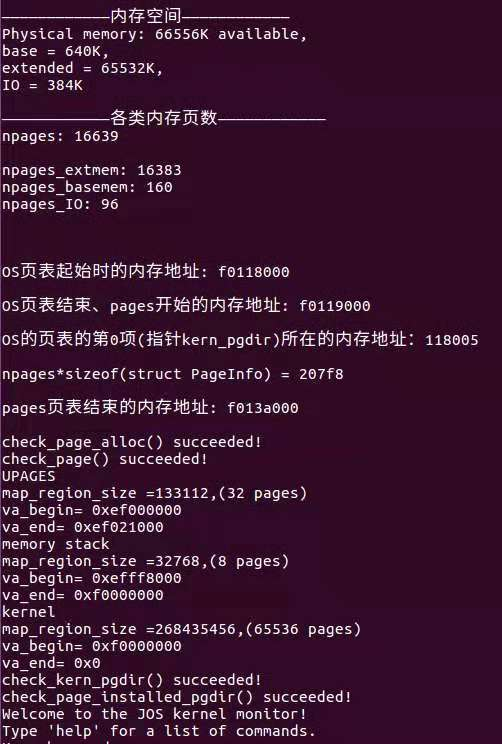
\includegraphics[width=0.8\linewidth]{figure/make_qemu}
\end{figure}

\begin{figure}[H]
\centering
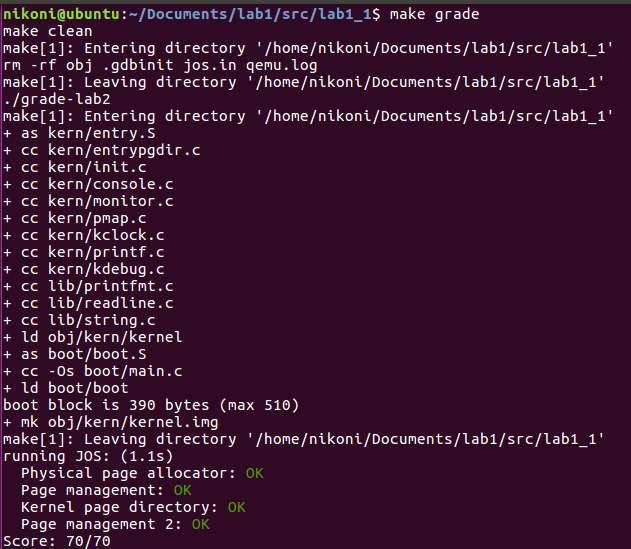
\includegraphics[width=0.8\linewidth]{figure/make_grade}
\end{figure}

\subsubsection{Question \Rmnum{4}}
\begin{flushleft}
1)\\
What entries (rows) in the page directory have been filled in at this point? What addresses do they map and where do they point? In other words, fill out this table as much as possible:
\begin{figure}[H]
\centering
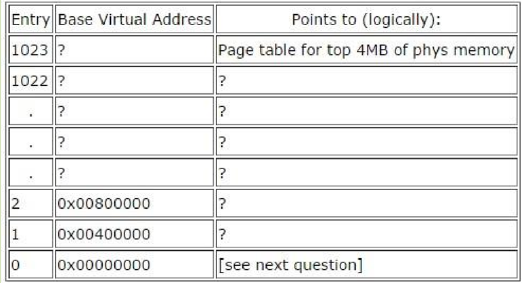
\includegraphics[width=0.8\linewidth]{figure/question4}
\end{figure}
\end{flushleft}
\begin{flushleft}
{\Large Answer}
\end{flushleft}
\begin{table}[H]
\centering
\begin{tabular}{ |p{150pt}<{\centering}|p{150pt}<{\centering}|p{150pt}<{\centering}| }\toprule
\hline				
Entry & Base Virtual Address &Points to(logically) \\ \hline 	
1023 & 0xffc00000 Points to(logically) & Page table for top 4MB of physical memory.This is the last address finding page table that the kernel can use.\\ \hline
1022 & 0xff800000 &Page table for 248MB--(252MB-1)physical memory \\ \hline 	
... & ... &Page table for physical memory \\ \hline
960 & 0xf0000000(KERNBASE) &static data 0--(4MB-1) physical memory \\ \hline
959 & 0xefc00000(VPT) &Page directory self (kernel RW).This is the first page table and it ’ s in the bottom of the physical memory. \\ \hline
958 & 0xef800000(ULIM) &Page table for kernel stack.It is mapped into the physical memory which is the same as bootstack.We only map the memory that the same as KSTACKSIZE.The rest memory that wasn’t mapped is used to avoid the overflow of the kernel stack. \\ \hline
957 & 0xef400000(UVPT) &Same as 959(user kernel R) \\ \hline
956 & 0xef00000(UPAGES) &Page table for structure pages[] \\ \hline
... & ... & NULL \\ \hline
2 & 0x00800000 & NULL \\ \hline
1 & 0x00400000 & NULL \\ \hline
0 & 0x00000000 & The start of the virtual memory .The same as 960(then turn to NULL)\\ \hline
\end{tabular}
\caption{Answer}
\end{table}

\begin{flushleft}
2)We have placed the kernel and user environment in the same address space. Why will user programs not be able to read or write the kernel's memory? What specific mechanisms protect the kernel memory?

{\Large Answer}
\end{flushleft}

User is not allowed to access kernel memory for safety reasons.
If user have the permission, bugs in user code may led to crash.
It is the paging mechanism that protects kernel address in JOS. If the flag bit PTE\_U is 0 in a page, that means user have no permission to read or write the page.

\begin{flushleft}
3)What is the maximum amount of physical memory that this operating system can support? Why?

{\Large Answer}
\end{flushleft}
\begin{figure}[H]
\centering
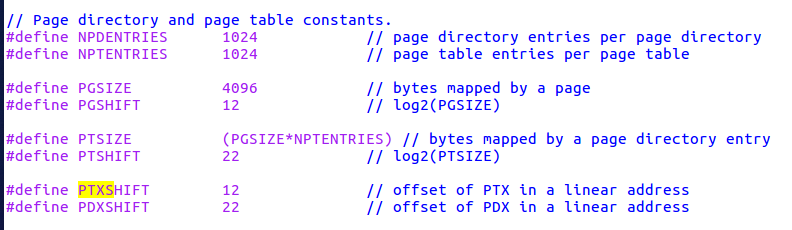
\includegraphics[width=0.8\linewidth]{figure/question4_3_1}
\caption{PTSIZE}
\end{figure}

\begin{figure}[H]
\centering
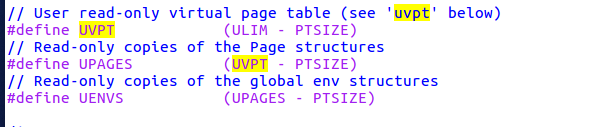
\includegraphics[width=0.8\linewidth]{figure/question4_3_2}
\caption{UPAGES}
\end{figure}

\begin{figure}[H]
\centering
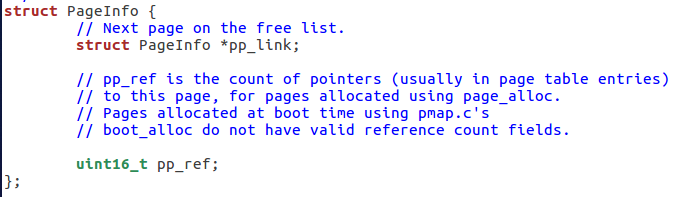
\includegraphics[width=0.8\linewidth]{figure/question4_3_3}
\caption{Page}
\end{figure}

2GB.

Pages use up to 4MB space, and each PageInfo use 8Byte. 4M / 8 * 4kB=2GB (4kB per page).


\begin{flushleft}
4)How much space overhead is there for managing memory, if we actually had the maximum amount of physical memory? How is this overhead broken down?

{\Large Answer}
\end{flushleft}

The total overhead to manage maxium amount of physical memory is:

  786432 bytes (struct Pages [1])

  4096 bytes (one page directory [2])

  262144 bytes (64 page tables [3])

  ------------

  1052672 bytes (~1MB)

  The only way I can see to reduce that amount is to use 4MB pages, this
  would reduce the struct Page allocations to 768 bytes and no need to
  allocate page tables.

  On the hand, the greater the granularity the greater the amount of
  unused chunks we'll have on the allocated pages which means we'll
  spend memory...

  [1] struct Page overhead was calculated this way
  256 * 1024 * 1024 / 4096 * 12
  256MB Page size size of struct Page

  [2] Page directory is 4096 bytes long by definition

  [3] Page table overhead was calculated this way

  (256 * 1024 * 1024 / (4096 * 1024)) * 4096
  256MB PG maps 4MB PG size
\clearpage
